\section{DATA PREDICTIVE CONTROL}
\label{S:dpc}

\textcolor[rgb]{0,0,1}{The central idea behind DPC is to obtain control-oriented models using machine learning on historical datasets of buildings and formulate the optimal control problem in a way that Receding Horizon Control (RHC) can be solved efficiently. Let an historical dataset $(\X,\Y)$ be given.
We define $\X = \{(x(k),u(k),d(k))\}_{k=1}^n$ the set of predictor variables (or features), i.e. the set of samples $(x(k),u(k),d(k))$ measured a time instants $k=1,\ldots,n$, where $x(k)\in\mathbb{R}^{n_x}$ is the vector of the \emph{measurable} state variables (e.g. the rooms temperatures, power consumption of the building, and others), $u(k)\in\mathbb{R}^{n_u}$ is the vector of the \emph{measurable} input variables (e.g. the set-points and schedule information of the building) and $d(k)\in\mathbb{R}^{n_d}$ is the vector of the \emph{measurable and predictable} disturbance variables (e.g. weather historical data).
We define $\Y = \{y(k)\}_{k=1}^{n}$ the set of response variables, i.e. the set of measured samples $y(k)\in\mathbb{R}^{n_y}$ representing the variables we wish to predict with our model. In the most general case, when we want to predict all measured variables, the response variables are represented by the state variables at the next time step, i.e. $y(k) = x(k+1)$. However, in general, we only wish to predict a subset $y(k) = \bar x(k+1) \subset \mathbb{R}^{n_x}$ of variables, e.g. only room temperatures and power consumption.
Clearly, $|\X| = |\Y| = n$ is the number of time samples of the dataset.\\
We remark that, as explained in Section \ref{secModelingIssuesExample}, the dataset $(\X,\Y)$ does not contain non-measurable states such as temperature of wall layers, ceiling, floor, etc.: nevertheless, our simulated and experimental results show that our data-driven methodology is able to compensate the absence of such variables while providing excellent prediction accuracy.}

\textcolor[rgb]{0,0,1}{Our goal is to learn data-driven models, using Regression Trees and Random Forests, that relate the value of the response variables (possibly for a certain future time horizon) with the value of the predictor variables and can be used to set up an MPC problem. To this aim, in the simplest example of one time-step prediction, we need to derive a model with a closed-form expression of the following form
\begin{equation}\label{E:GenericModel}
	y(k)=x(k+1)=f(x(k),u(k),d(k)).
\end{equation}
However classical Regression Tree and Random Forest algorithms do not provide a closed-form expression for $f$, hence they cannot be used for MPC.}

\textcolor[rgb]{0,0,1}{In the next section we provide a new methodology (DPC) that adapts the classical Regression Tree and Random Forest algorithms to determine a closed-form expression for $f$ that is efficiently applicable to MPC. For simplicity of presentation we first describe DPC using Regression Trees and then DPC using Random Forests.}

%==============================================================================================================

\subsection{DPC-RT: DPC with Regression Trees}
\label{SS:dpcrt}

\textcolor[rgb]{0,0,1}{In order to have a model that can be used for prediction in an MPC problem with a future horizon of arbitrary length $N$	 we need to predict, at time $k$, the response $y$ for the next $N$ time steps, i.e. $y(k),\ldots,y(k+N)$. For the sake of simplicity and without loss of generality we consider in this section only a scalar response variable, i.e. $y(k)\in\mathbb{R}$ ($n_y = 1$). We will show in Sections \ref{S:casestudy} and \ref{S:realCaseStudy} that multiple trees (or forests) can be easily built to account for the case when $n_y > 1$.}

\textcolor[rgb]{0,0,1}{Assume that, at time $k$, we want to predict the response variable at time $k+j$, i.e. $y(k+j),\ j\in \{1,\ldots,N\}$: when the data have lots of features interacting in complicated, nonlinear ways, assembling a single global model such as linear or polynomial regression can be difficult, and can lead to poor response predictions.}

\textcolor[rgb]{0,0,1}{As discussed before an approach to non-linear regression is to partition the dataset into smaller regions where the interactions are more manageable. This partition can be obtained by recursively splitting the dataset via an adaptation we propose to the Regression Tree algorithm (see Appendix 1 for details), and is repeated recursively until we finally get to small chunks of the dataset (i.e. the leaves of the regression tree) where we can fit simple (e.g. linear or affine) parametric models.}

%Therefore, in \eqref{E:sepvars}, the global model $f$ has two parts: the recursive partition $g$, and a linear (and convex) model $h$ for each cell of the partition.

\begin{figure}[t!]
	\centering
	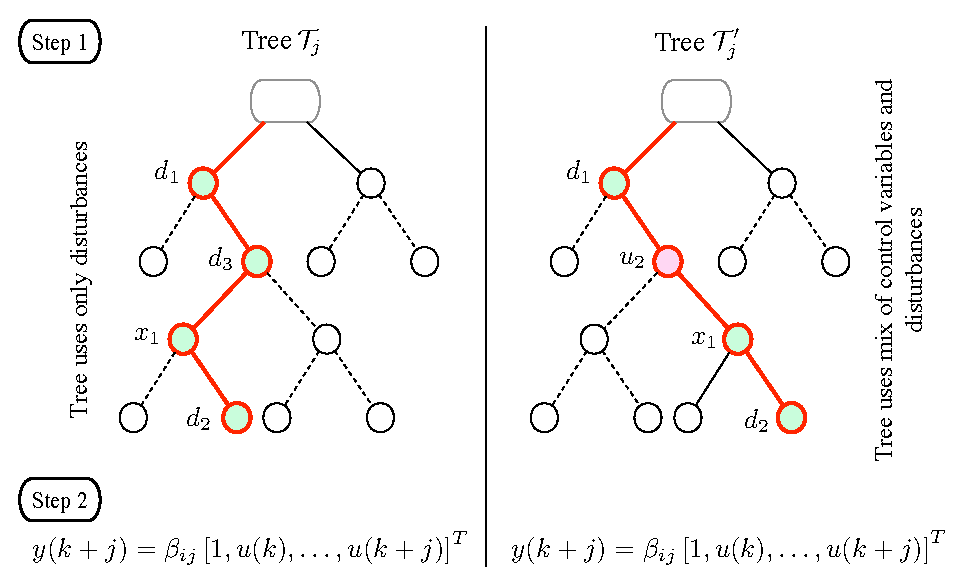
\includegraphics[width=20pc]{figures/dpc-sepvars.eps}
	\caption{\textit{Step 1:} Tree $\mathcal{T}_j$ trained only with variables in $\X^d$ using adapted RT algorithm. Tree $\mathcal{T}'_j$ trained with variables in $\X^d$ and control variables in $\X^c$ using classical RT algorithm. \textit{Step 2:} In the leaf $\ell_i$ of the tree an affine model $\beta_{ij}$ is defined as a function only of the control variables dataset corresponding to leaf $\ell_i$.}
	\captionsetup{justification=centering}
	\label{F:dpc-sepvars}
\end{figure}

\textcolor[rgb]{0,0,1}{Our modification of the Regression Tree algorithm first partitions the features set $\X$ into the sets $\X^c = \{u(k)\}_{k=1}^n\subset\X$, containing the control (or manipulated) variables, and $\X^d = \{(x(k),d(k))\}_{k=1}^n\subset\X$, containing the disturbance and state (or non-manipulated) variables. The  union of the two non-intersecting sets forms the full feature set of training $\X \equiv \X^c \cup \X^d$.
%Our goal is to replace a model-based controller with a data-driven controller, where the latter depends only on the historical sensor data. 
%These measurements could directly represent one or more states in the model-based control framework. We denote these as responses $\Y \in \R$ for training, i.e. a $\Y$ represents a particular response and we can have separate models for multiple responses. We define the number of training samples by $|(\X,\Y)| = n$.
Then the training process is divided into the following two steps, which generate as output a tree $\mathcal{T}_j$ as illustrated in Figure~\ref{F:dpc-sepvars} (left):
\begin{enumerate}
	\item the splitting of the dataset only partitions $\X^d$ (see Appendix 1 and \cite{hastie2009elements} for technical details): this choice is necessary to make our model suitable for control, as we will clarify later on, and also reduces the computational complexity. To each leaf $\ell_i$ will correspond an equivalence class of data samples $\X^d_i$ of the partition of $\X^d$, with $\X^d_i\subset \X^d$: as a consequence at any time $k$, given $\delta_d$ autoregressive terms of the disturbances and $\delta_x$ autoregressive terms of the state, we can associate $( d(k-\delta_d),\ldots,d(k+j),x(k-\delta_x),\ldots,x(k) )$, to the corresponding leaf $\ell_i$
	\begin{equation}\label{E:model_tree}
		\ell_i = \mathit{g}_{\mathcal{T}_j} \left( d(k-\delta_d),\ldots,d(k+j),x(k-\delta_x),\ldots,x(k)  \right)
	\end{equation}
	if and only if $( d(k-\delta_d),\ldots,d(k+j),x(k-\delta_x),\ldots,x(k)) \in \X^d_i$.
	\item in each leaf $\ell_i$ of the tree $\mathcal{T}_j$ we derive, solving a convex program over the data samples in the partition $\X^d_i$ associated to leaf $\ell_i$, an affine function, with coefficients $\beta_{ij}$, that relates the response $y(k+j)$ to the previous control inputs in $\X^c$:
	\begin{equation}\label{E:model_leaf}
		y(k+j) =  \beta_{ij} [1,u(k),\ldots,u(k+j) ]^T
	\end{equation}
	Clearly the coefficients $\beta_{ij}$ are different for each leaf $\ell_i$ as they are derived from different sets of samples.
\end{enumerate}
As an example, the tree $\mathcal{T}_0$ defines the function $f$ in \eqref{E:GenericModel} to predict $y(k)$ as follows: assuming for simplicity that $\delta_x = \delta_d = 0$, given the measurement of the variables $(x(k), d(k))$ at time $k$, it is possible to determine by \eqref{E:model_tree} the corresponding leaf $\ell_i$ of $\T_0$ and the associated $\beta_{i0}$. The prediction of $y(k)$ is provided by \eqref{E:model_leaf} as an affine function of the control variable $u(k)$.\\
Applying the above procedure for $j=0,\ldots,N$, we build $N$ regression trees $\mathcal{T}_0,\ldots,\mathcal{T}_N$: thus, we have managed to linearize the original model dynamics via black-box modeling.\\ 
Our two-steps training procedure, described by the pseudo code of lines 1-11 of Algorithm~\ref{A:dpcrt}, can be computed off-line: this is an important advantage because the time required to create the model does not affect the control execution in run-time.}

\textcolor[rgb]{0,0,1}{The next problem now is: \emph{how to use this modeling framework to set up an MPC problem?} We setup the MPC optimization problem in the general case of multiple responses, i.e. $y(k)\in\mathbb{R}^{n_y},\ n_y\geq 1$, as follows:}
\begin{problem}\label{P:dpcrt}
	\begin{equation}
		\begin{aligned}
		& \underset{u_{k+j},\epsilon_j}{\mathrm{minimize}} & & \sum_{j=0}^{N} y^\top_{k+j} Q y_{k+j} + u^\top_{k+j} R u_{k+j} + \lambda\epsilon_j \\
		& \mathrm{subject\ to }                 & & y_{k+j}     =   \hat \beta_{j} [1,u^\top_{k},\ldots,u^\top_{k+j} ]^\top                       \\
		&                                       & & u_{k+j}    \in  \mathcal{U}                                                                   \\
		&                                       & & |y_{k+j}|  \leq \bar{y}_{k+j} + \epsilon_j 										              \\
		&                                       & & \epsilon_j \geq  0							                                                  \\
		&                                       & & j           =    0,\ldots,N,               									                  \\
		\end{aligned}
		\label{E:dpcrt}
	\end{equation}
\end{problem}

\noindent \textcolor[rgb]{0,0,1}{where $\hat \beta_j$ is defined later on. Here, $Q \succeq 0 \in \mathbb{R}^{n_y\times n_y}$ and $R \succeq 0 \in \mathbb{R}^{n_u\times n_u}$ are weight matrices used to trade-off the importance we provide in the minimization to $y$ versus $u$. The slack variables $\epsilon_j$ are added to ensure recursive feasibility: we relax the equality constraint on $y$ allowing violation up to $\epsilon_j$ to guarantee that Problem \ref{P:dpcrt} can provide a solution at each step $k \geq 0$. The weight $\lambda$ is then used to tradeoff the importance we provide in the optimal solution to the constraints violation versus the quadratic term. For example in the following sections we will use $\epsilon_j$ and $\lambda$ to define our tolerance to the violation of prescribed bounds by the rooms' temperature.\\
Clearly different cost functions can be chosen depending upon the application, i.e. they can be linear, nonlinear, etc., obviously changing the complexity of the problem. In the current formulation, the data-driven control problem, is reduced to a convex program which is very easy and efficient to solve in C, C++, Python and Matlab, and thus is easily integrable in SCADA systems.
Indeed, Problem \ref{P:dpcrt} is solved as in the classical MPC formulation, i.e. at each time step $k=1,2,\ldots$ the optimal control sequence $u^*_k,\ldots,u^*_{k+N}$ is computed, and only the first input of the sequence is applied to the system: $u(k) = u^*_k$.\\
Note that each tree $\T_j$ contributes to Problem  \ref{P:dpcrt} with the linear constraint $y_{k+j} = \hat \beta_{j} [1,u^\top_{k},\ldots,u^\top_{k+j} ]^\top$ as a replacement for the state dynamics in the classical MPC formulation. As a consequence, when solving Problem \ref{P:dpcrt} at time $k$, we need to determine the affine functions parameters $\hat \beta_{j}$: it follows by Equation \eqref{E:model_tree} that, to determine $\beta_{ij}, j=0,\ldots,N$ at time $k$, the knowledge of the state and disturbance measurements $\left( d(k-\delta_d),\ldots,d(k+N),x(k-\delta_x),\ldots,x(k) \right)$ is needed. However, the values of $d(k+1),\ldots,d(k+N)$ are not available at time $k$, so we need to use disturbance forecast $\tilde d(k+1),\ldots,\tilde d(k+N)$. Using this information we can narrow down to a leaf in each tree using \eqref{E:model_tree} and thus retrieve the affine model with $\beta_{ij}$ in \eqref{E:model_leaf} for each step $j=0,\ldots,N$ of the horizon, and associate $\hat \beta_j := \beta_{ij}$. The run-time solution of Problem \ref{P:dpcrt} illustrated above is described by the pseudo code of lines 12-23 of Algorithm~\ref{A:dpcrt}.}

\textcolor[rgb]{0,0,1}{\begin{remark}
The authors in \cite{Petersen2014AE} investigate the effect of uncertainty in the weather forecast on the performance of MPC in building systems operations through a large-scale simulation study, and compare against a rule-based strategy. They consider 48 different scenarios of uncertainties for 72 hours weather forecast. With such a long horizon, results have shown that (with a few exceptions) MPC outperforms the rule-based controller in providing energy savings, and is in general quite close to the perfect forecast case despite the uncertainty in weather forecast. The length of horizon for the DPC algorithm presented in this paper is usually much shorter, for example $6$ hours in Section \ref{S:proof}, $7$ hours in Section \ref{S:casestudy}, and $40$ minutes in Section \ref{S:realCaseStudy}. As a consequence, we can reasonably presume that our approach will be robust to weather forecast inaccuracies. Indeed, in Section \ref{S:realCaseStudy} we test the robustness of our approach to noisy weather forecast and show that the control performance is very close to the ideal case.
%This means the weather forecast is more accurate than the 72 hours case presented in \cite{Petersen2014AE}, hence also control performance is even closer to the perfect knowledge forecast case.
\end{remark}}

\textcolor[rgb]{0,0,1}{\begin{remark}
It is now easy to understand that using the classical Regression Tree algorithm, e.g. using also the input variable $u$ in the data splitting procedure to create the trees as in the right side of Figure~\ref{F:dpc-sepvars}, the resulting model would not be suitable for control. Indeed, since $u$ is the variable we want to optimize in Problem \ref{P:dpcrt}, at time $k$ we have still not chosen its value at times $k, \ldots, k+N$: as a consequence the affine functions \emph{parameters }$\beta_{ij}$ needed to set up Problem \ref{P:dpcrt} cannot be determined at time $k$.
\end{remark}}

\textcolor[rgb]{0,0,1}{The pseudo code for the whole DPC-RT procedure (i.e. Off-line and Run-time) is given in Algorithm~\ref{A:dpcrt}. Our procedure is also graphically described in Figure \ref{F:dpc-algo-rf} for the Random Forest case, providing a good intuition also for the Regression Tree case.}

\textcolor[rgb]{0,0,1}{\begin{algorithm}[ht!]
	\caption{Data Predictive Control with Regression Trees}
	\label{A:dpcrt}
	\begin{algorithmic}[1]
		\State \textsc{Design Time (Off-Line)}
		\Procedure{Model Training using Dataset Splitting}{}
		\State Set $\X^c$ $\gets$ manipulated features
		\State Set $\X^d$ $\gets$ non-manipulated features
		\State Build $N$ predictive trees with $(\X^d,\Y)$ using Regression Trees algorithm
		\ForAll{trees $\mathcal{T}_j$}
		\ForAll{leaves $\ell_i$ of $\mathcal{T}_j$}
		\State Compute parameters $\hat\beta_j:=\beta_{ij}$ in \eqref{E:model_leaf} using convex programming
		\EndFor
		\EndFor
		\EndProcedure
		\State \textsc{Run Time}
		\Procedure{Predictive Control}{}
		\While{$k< k_{\mathrm{stop}}$}
		\ForAll{trees $\mathcal{T}_j$}
		\State Determine the leaf $\ell_i$ using $\X^d$ as in \eqref{E:model_tree}
		\State Obtain the linear model at $\ell_i$ trained in \eqref{E:model_leaf}
		\EndFor
		\State Solve Problem \ref{P:dpcrt} to determine optimal
		\State control actions $u^*_k,\ldots,u^*_{k+j}$
		\State Apply the first input $u(k)=u^*_k$
		\EndWhile
		\EndProcedure
	\end{algorithmic}
\end{algorithm}}

%==============================================================================================================

\subsection{DPC-En: DPC with Ensemble Methods}
\label{SS:dpcrf}

\textcolor[rgb]{0,0,1}{Regression trees obtain good predictive accuracy in many domains. However, the models used in their leaves have some limitations regarding the kind of functions they are able to approximate. The problem with trees is their high variance and that they can overfit the data easily, and a small change in the data can result in a different series of splits and thus affect the prediction accuracy. This is the price to be paid for estimating a tree-based structure from the data.}

\textcolor[rgb]{0,0,1}{To address the above problems we use ensemble methods \cite{Friedman2001}, in particular Random Forests, to combine the predictions of several independent regression trees in order to improve generalizability and robustness over a single estimator. The essential idea is to average many noisy trees to reduce the overall variance in prediction. We inject randomness into the tree construction in two ways: first, we randomize the features used to define splitting in each tree; second, we build each tree using a bootstrapped or sub-sampled data set. As a consequence each tree in the forest is trained on different data, which introduces differences between the predictive models of the trees.}

\textcolor[rgb]{0,0,1}{More precisely, in DPC-En we replace each tree in Algorithm~\ref{A:dpcrt} by a forest $\F_j$ of $t$ trees $\T_{1j},\ldots,\T_{tj}$. Each tree $\T_{\kappa j}$ is trained on the basis of a different subset of features $\bar{\X}^d_{\kappa j} \subset \X^d$. As discussed in the previous section, at any time $k$, given $\delta_d$ autoregressive terms of the disturbances and $\delta_x$ autoregressive terms of the state, we can associate $( d(k-\delta_d),\ldots,d(k+j),x(k-\delta_x),\ldots,x(k) )$, to the corresponding leaf $\ell_i$ of $\T_{\kappa j}$
\begin{equation}\label{E:model_forest}
	\ell_i = \mathit{g}_{\mathcal{T}_{\kappa j}} \left( d(k-\delta_d),\ldots,d(k+j),x(k-\delta_x),\ldots,x(k)  \right).
\end{equation}
Also, in each leaf $\ell_i$ of tree $\mathcal{T}_{\kappa j}$ we derive an affine function $\Theta_{i \kappa j}$, that relates the response $y(k+j)$ to the previous control inputs in $\X^c$:
\begin{equation}\label{E:model_leaf_forest}
	y(k+j) =  \Theta_{i \kappa j} [1,u(k),\ldots,u(k+j) ]^T.
\end{equation}
}

%In particular, as mentioned above, each tree $\T_i$ of each forest $\F_j$ is trained using $(\bar \X^d_i,\bar\Y_i)$.
%Here $(\bar\X^c_i,\bar\Y_i)$ correspond to the in-bag samples for the trees.

\textcolor[rgb]{0,0,1}{We can now set up the MPC problem for DPC-En as follows:}
\begin{problem}\label{P:dpcrf}
	\begin{equation}
		\begin{aligned}
		& \underset{u_{k+j},\epsilon_j}{\mathrm{minimize}} & & \sum_{j=0}^{N} y^\top_{k+j} Q y_{k+j} + u^\top_{k+j} R u_{k+j} + \lambda\epsilon_j \\
		& \mathrm{subject\ to }                 & & y_{k+j}      =  \hat{\Theta}_{j} [1,u_{k},\ldots,u_{k+j} ]^\top                      \\
		&                                       & & u_{k+j}    \in  \mathcal{U}                                                        \\
		&                                       & & |y_{k+j}|  \leq \bar{y}_{k+j} + \epsilon_j 										 \\
		&                                       & & \epsilon_j \geq  0							                                     \\
		&                                       & & j           =    0,\ldots,N,            									         \\
		\end{aligned}
		\label{E:dpcrf}
	\end{equation}
\end{problem}

\noindent \textcolor[rgb]{0,0,1}{where $\hat{\Theta}_{j}$ is defined later on. Note that, as in the DPC-RT, the crucial problem when solving Problem \ref{P:dpcrf} is determining all parameters $\hat{\Theta}_{j}$ at time $k$. We first proceed similarly to DPC-RT by using forecast of disturbances and the state measurements to determine for each tree $\T_{\kappa j}$ the corresponding leaf $\ell_i$ and thus the affine model $\Theta_{i \kappa j}$, with $\kappa = 1,\ldots,t$ and $j = 0,\ldots,N$. In DPC-En, however, we have $t$ affine models for each prediction step $j$, thus we define $\hat{\Theta}_{j} = \frac{1}{t}\sum\limits_{\kappa = 1}^{t} \Theta_{i \kappa j}$ averaging the affine models associated to all trees of forest $\F_j$. Once we are able to determine at each time $k$ the parameters $\hat{\Theta}_{j}$ of the constraints of Problem \ref{P:dpcrf}, the optimal input $u^*_k$ can be computed as described in the previous section. The overall procedure is sketched in Figure \ref{F:dpc-algo-rf}.}
\begin{figure}[t!]
	\centering
	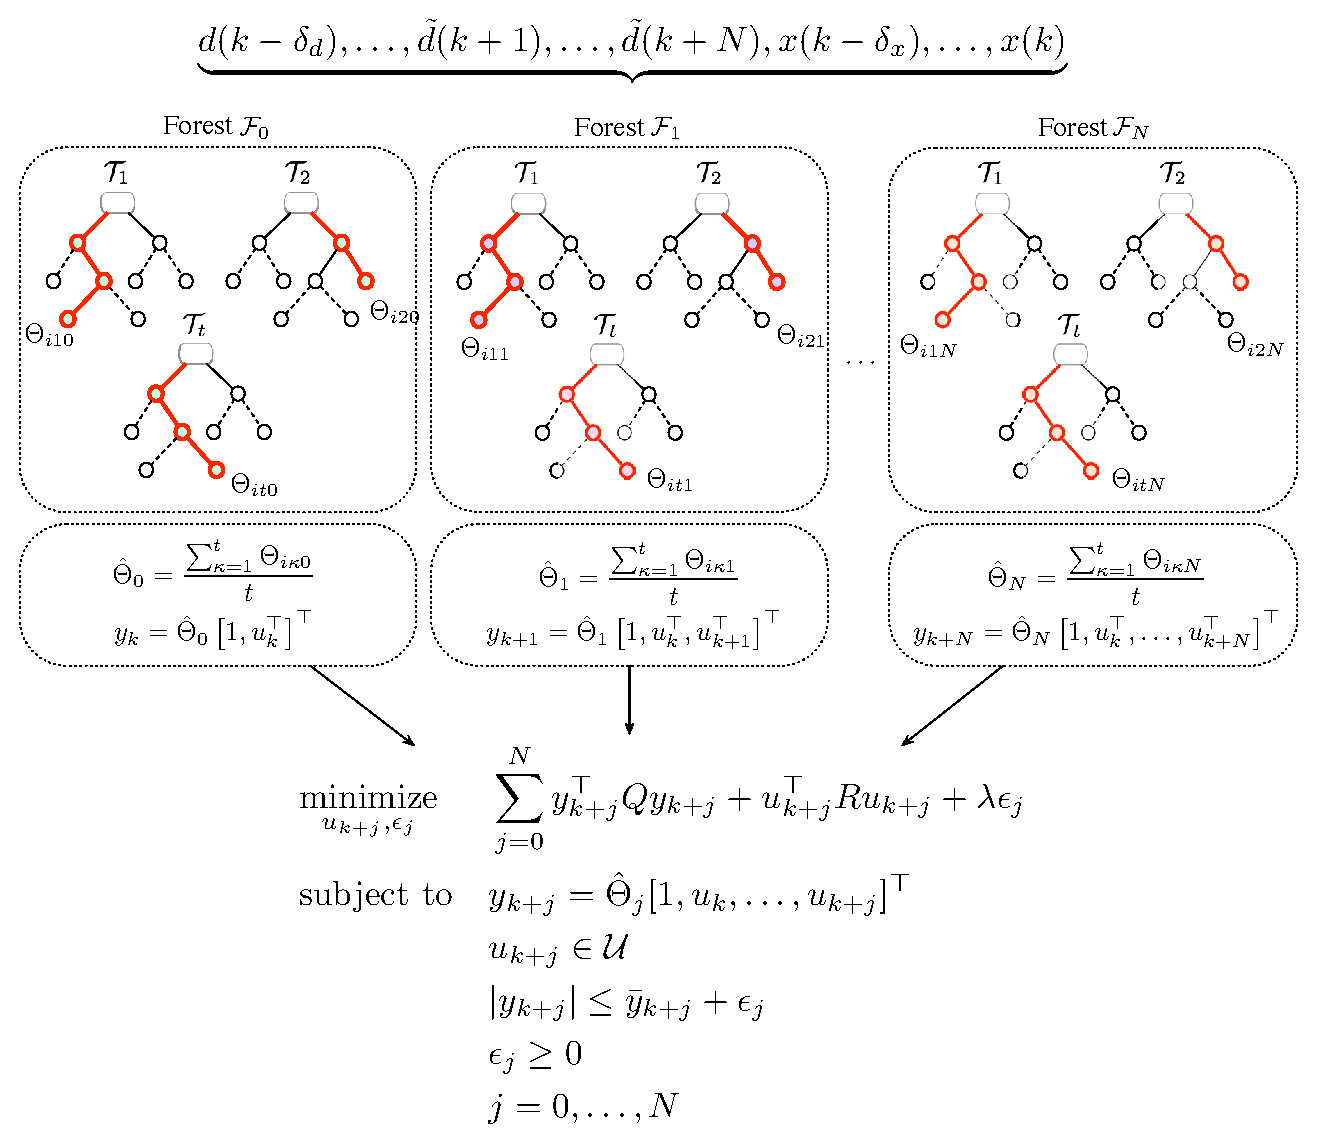
\includegraphics[width=26pc]{figures/dpc-algo-rf.eps}
	\caption{\textcolor[rgb]{0,0,1}{Graphical description of the procedure for solving Problem \ref{P:dpcrf} at each time $k$}}
	\label{F:dpc-algo-rf}
\end{figure}

\textcolor[rgb]{0,0,1}{The ensemble data predictive control (DPC-En) is the first such method to bridge the gap between ensemble predictive models (such as random forests) and receding horizon control. Reasoning on complexity, we remark that the off-line training computation in DPC-En is increased compared to DPC-RT as we need to train $t$ trees for each of the $N$ prediction steps. The run-time computation is also slightly increased as we need to derive the average $\hat{\Theta}_{j} = \frac{1}{t}\sum\limits_{\kappa = 1}^{t} \Theta_{i \kappa j}$ for each of the $N$ prediction steps. However, as shown in the following sections, it's worth the price as we obtain much better accuracy and lower variance properties with a marginal increase of the run-time computation time (the increase of off-line computation time is not a big issue as it must be run very seldom, i.e. only when a new model of the building needs to be created).}

